\documentclass{article}
\usepackage{graphicx} % Required for inserting images
\usepackage{amsmath}
\usepackage{amssymb}
\usepackage{float}
\usepackage{textgreek}
\usepackage{fancyhdr}
\usepackage{hyperref}
\usepackage{tikz}
\usetikzlibrary{shapes,arrows}
\usepackage{enumerate}

% vnořené popisky obrázků
\usepackage{subcaption}

% automatická konverze EPS 
\usepackage{graphicx} 
\usepackage{epstopdf}

\pagestyle{fancy}


\newcommand\mat[1]{\begin{bmatrix}#1\end{bmatrix}}
\newcommand\pdiff[2]{\frac{\partial #1}{\partial #2}}




\tikzstyle{block} = [draw, rectangle, minimum height=3em, minimum width=3em]
\tikzstyle{sum} = [draw, circle, node distance=1cm]
\tikzstyle{input} = [coordinate]
\tikzstyle{output} = [coordinate]
\tikzstyle{pinstyle} = [pin edge={to-,thin,black}]
\tikzstyle{tmp} = [coordinate] 





\title{ARI-HW\_07}
\author{Matěj Pinkas}
\date{5. April 2024}

\lhead{Pinkas Matěj}
\chead{ARI-HW\_07}
\rhead{5. April 2024}

\begin{document}

\maketitle

\section{Příklad}
\begin{itemize}
    \item Uvažujeme soustavu s přenosem otevřené smyčky:
    \begin{align*}
        L(s) = K\frac{1}{s(s+50)(5+100)}
    \end{align*}

    \item Zadaná soustava:
    \begin{figure}[h]
        \centering
        
        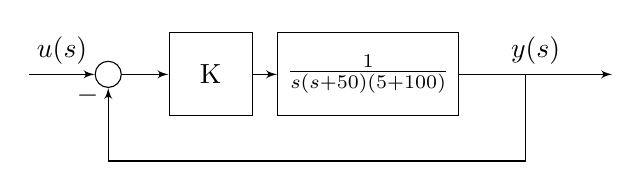
\begin{tikzpicture}[auto, node distance=1.1cm,>=latex']
            \node [input, name=input] {};
            \node [sum, right of=input] (sum1) {};
            \node [block, right of=sum1,node distance=1.3cm] (K) {K};
            \node [block, right of=K,node distance=2cm] (F) {$\frac{1}{s(s+50)(5+100)}$}; 
            \node [tmp, right of=F, node distance=2cm] (tmp1) {};
            \node [output, right of=tmp1] (output) {};
            \node [tmp, below of=K] (tmp2) {};
            
            \draw [draw,->] (input) -- node {$u(s)$} (sum1);
            \draw [->] (sum1) -- node {} (K);
            \draw [->] (K) -- node {} (F);
            \draw [->] (F) -- node [name=y] {$y(s)$}(output);
            \draw [->] (tmp1) |- (tmp2)-| node[pos=0.95] {$-$} (sum1);
        \end{tikzpicture}
    
        \caption{Systém s otevřenou smyčkou $L(s)$}
        \label{fig:System_1}
    \end{figure}
\end{itemize}

\begin{enumerate}[a)]
    \item Použití frekvenční metody k návrhu zesílení tak, aby měl výsledný zpětnovazební systém (uzavřená smyčka) překmit na skok reference: $20\%$
    \begin{align*}
        OS_\% &= 20\% & OS &= 0,2
    \end{align*}
    \begin{align*}
        \zeta = -\frac{\ln{(OS)}}{\sqrt{\pi^2+\ln{(OS)}^2}} \approx - \frac{-1,60944}{\sqrt{\pi^2+2,59029}} \approx 0,45595
    \end{align*}
    \begin{align*}
        PM = \arctan{\left(\frac{2\zeta}{\sqrt{-2\zeta^2+\sqrt{1+4\zeta^4}}}\right)} \approx 0,840337 \ \mathbf{rad}
    \end{align*}
    - Pomocí PM určíme amplitudu, tuto amplitudu hledáme na Bodeho grafu kde vyčteme frekvenci pro tuto amplitudu $\omega_{PM}$

    \begin{figure*}[hbt]
        \centering
        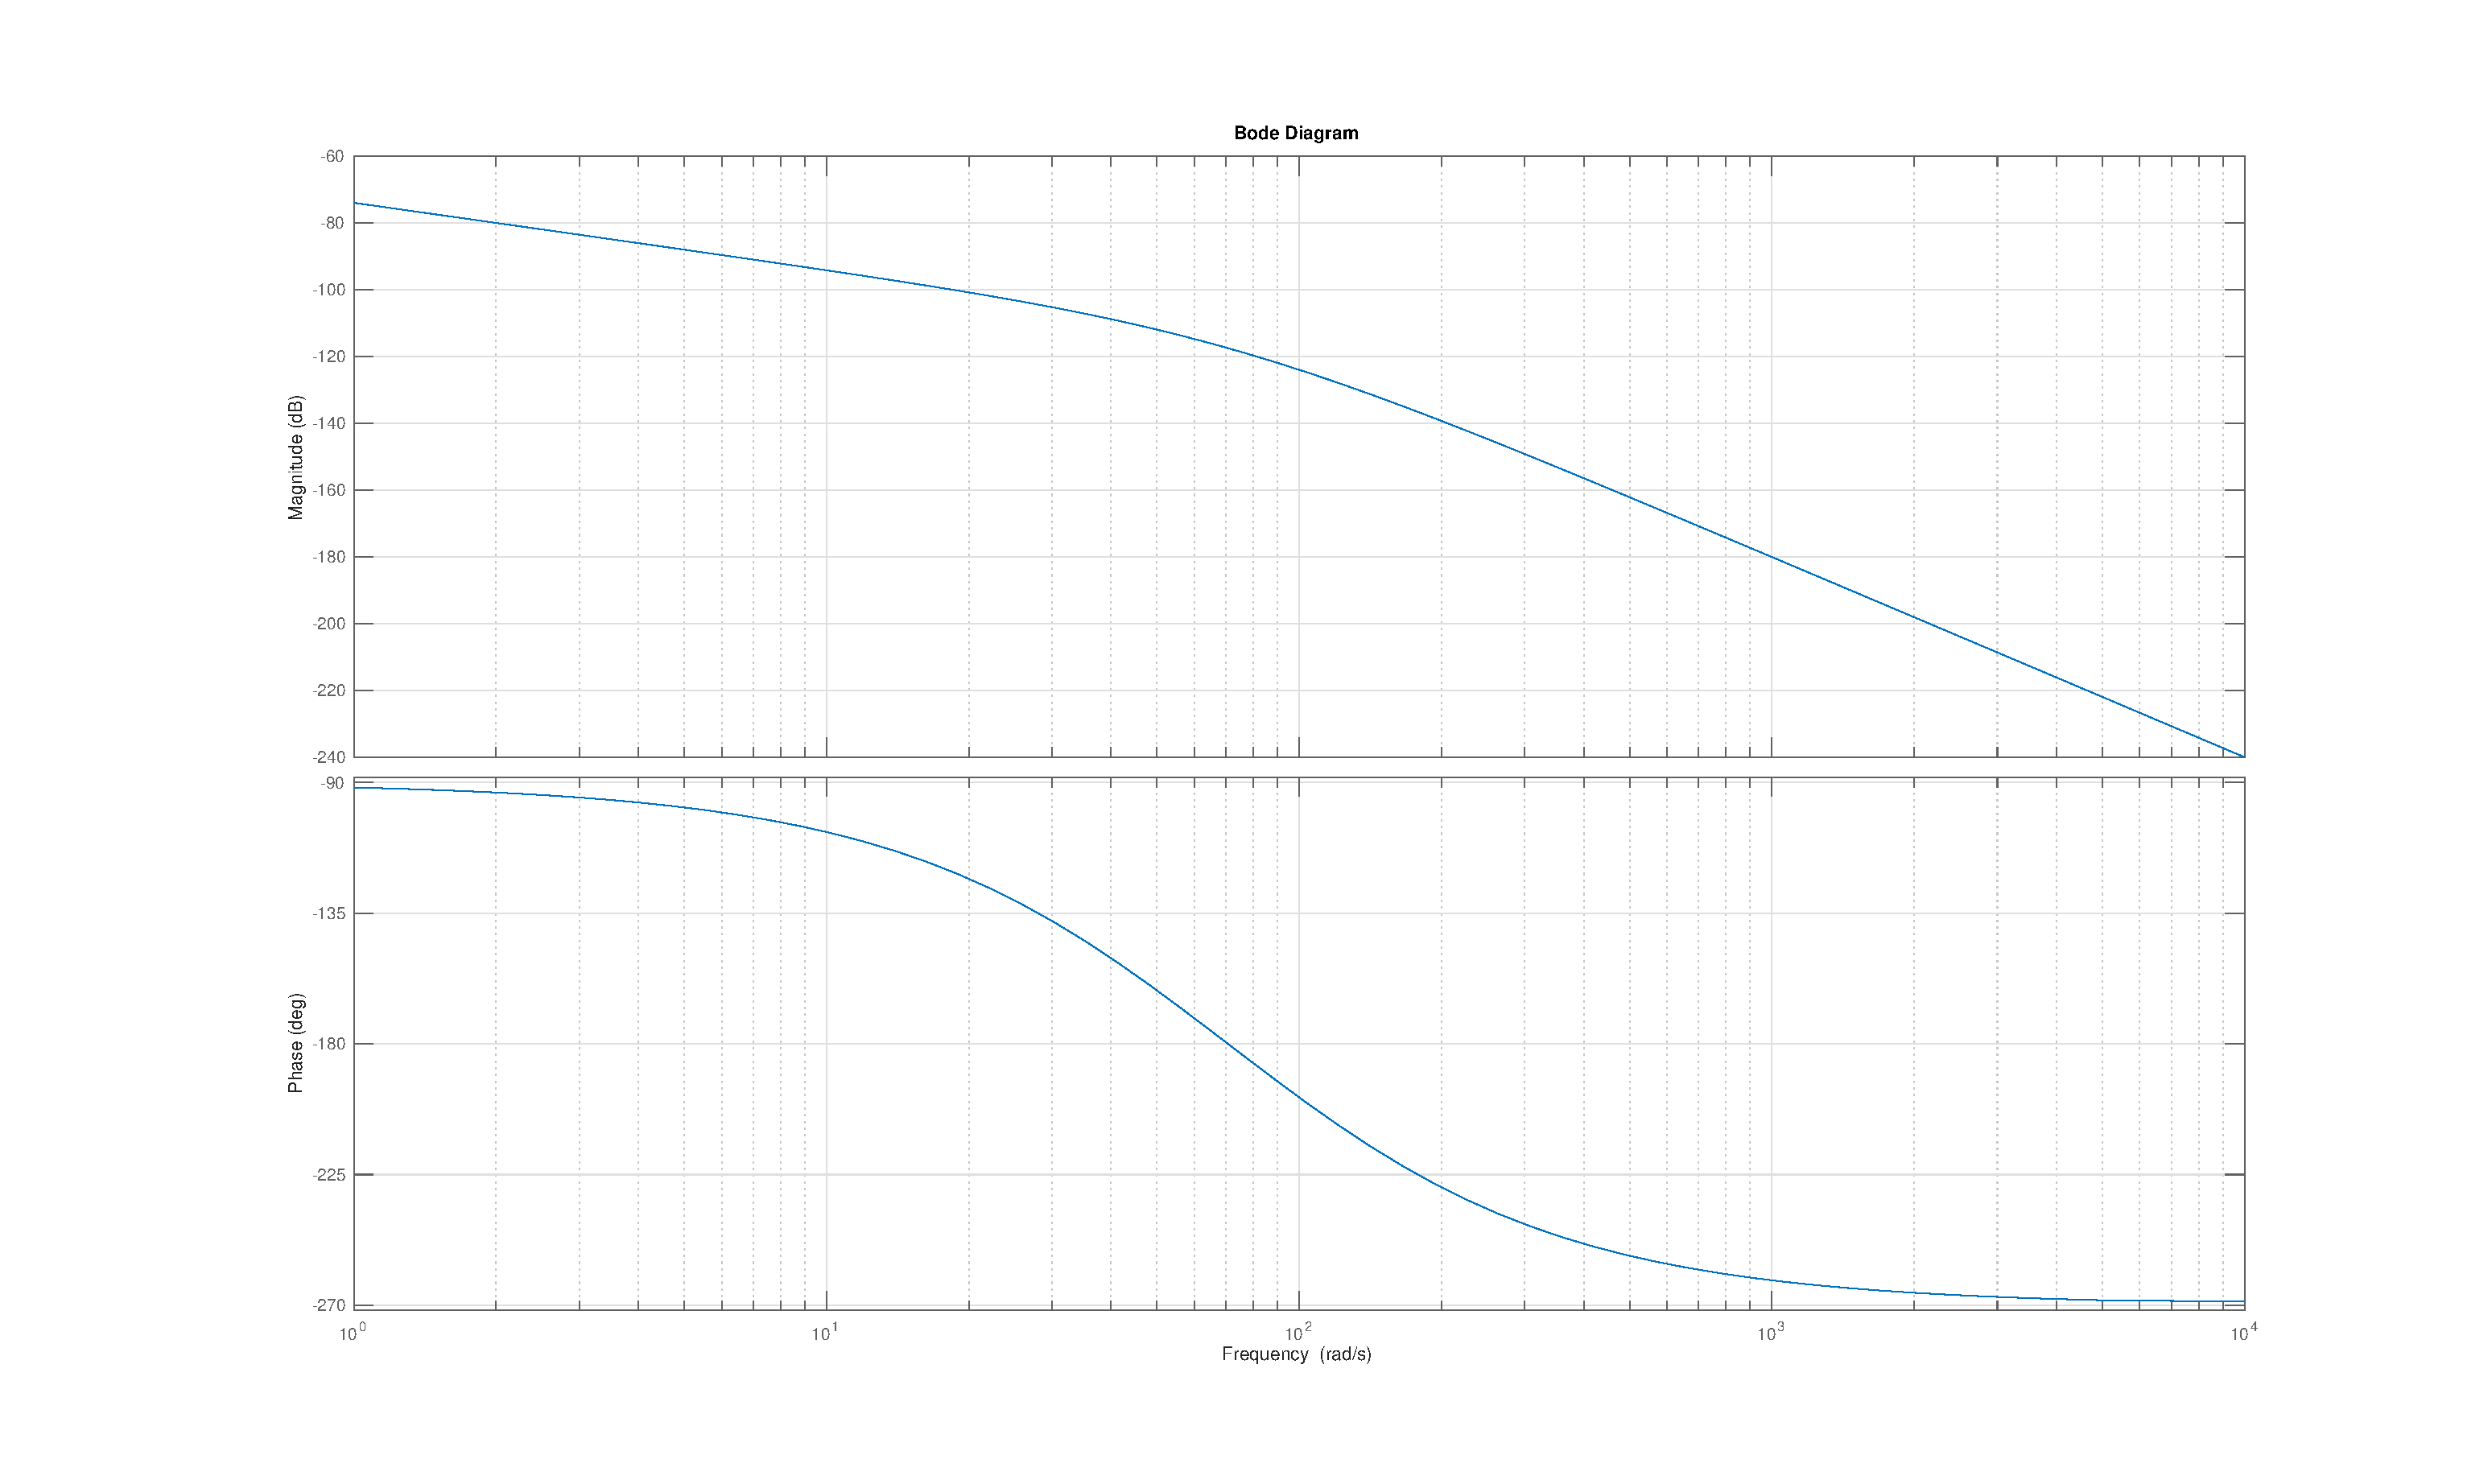
\includegraphics[clip, width=0.5\textwidth]{Bode_Plot.eps}
        \caption{Konstanta z Bodeho grafu}
        \label{fig:Const_Bode}
    \end{figure*}
    
    \begin{align*}
        \text{Amplituda} \ \omega_{PM} &\dots - \pi + PM \approx -2,30126\\
        \omega_{PM} &= 25,4 \ \mathbf{rad/s}
    \end{align*}
    - Získanou frekvenci dosadíme do předpisu $L(s)$, tedy $L(j\omega)$\\
    - $L(j\omega)$ bude rovna 0 dB = 1\\
    - Upravením funkce získám odhad pro K
    \begin{align*}
        \left|L\left(j\omega_{PM}\right)\right| &= \left| \frac{K}{j\omega_{PM}\left( j\omega_{PM} + 50 \right) \left( j\omega_{PM} + 100 \right)} \right| = 1\\
        K &\approx 146970,8429
    \end{align*}

    \item Ověření simulací
    \begin{align*}
        L(s) &= K\frac{1}{s(s+50)(5+100)} = \frac{146970,8429}{s^3+150s^2+5000s}\\
        T(s) &= \frac{L(s)}{1+L(s)} = \frac{1,47 \cdot 10^5 s^3 + 2,205 \cdot 10^7 s^2 + 7,349 \cdot 10^8 s}{ s^6 + 300 s^5 + 32500 s^4 + 1,647 \cdot 10^6 s^3 + 4,705 \cdot 10^7 s^2 + 7,349 \cdot 10^8 s}
    \end{align*}

    \begin{figure*}[htb]
        \centering
        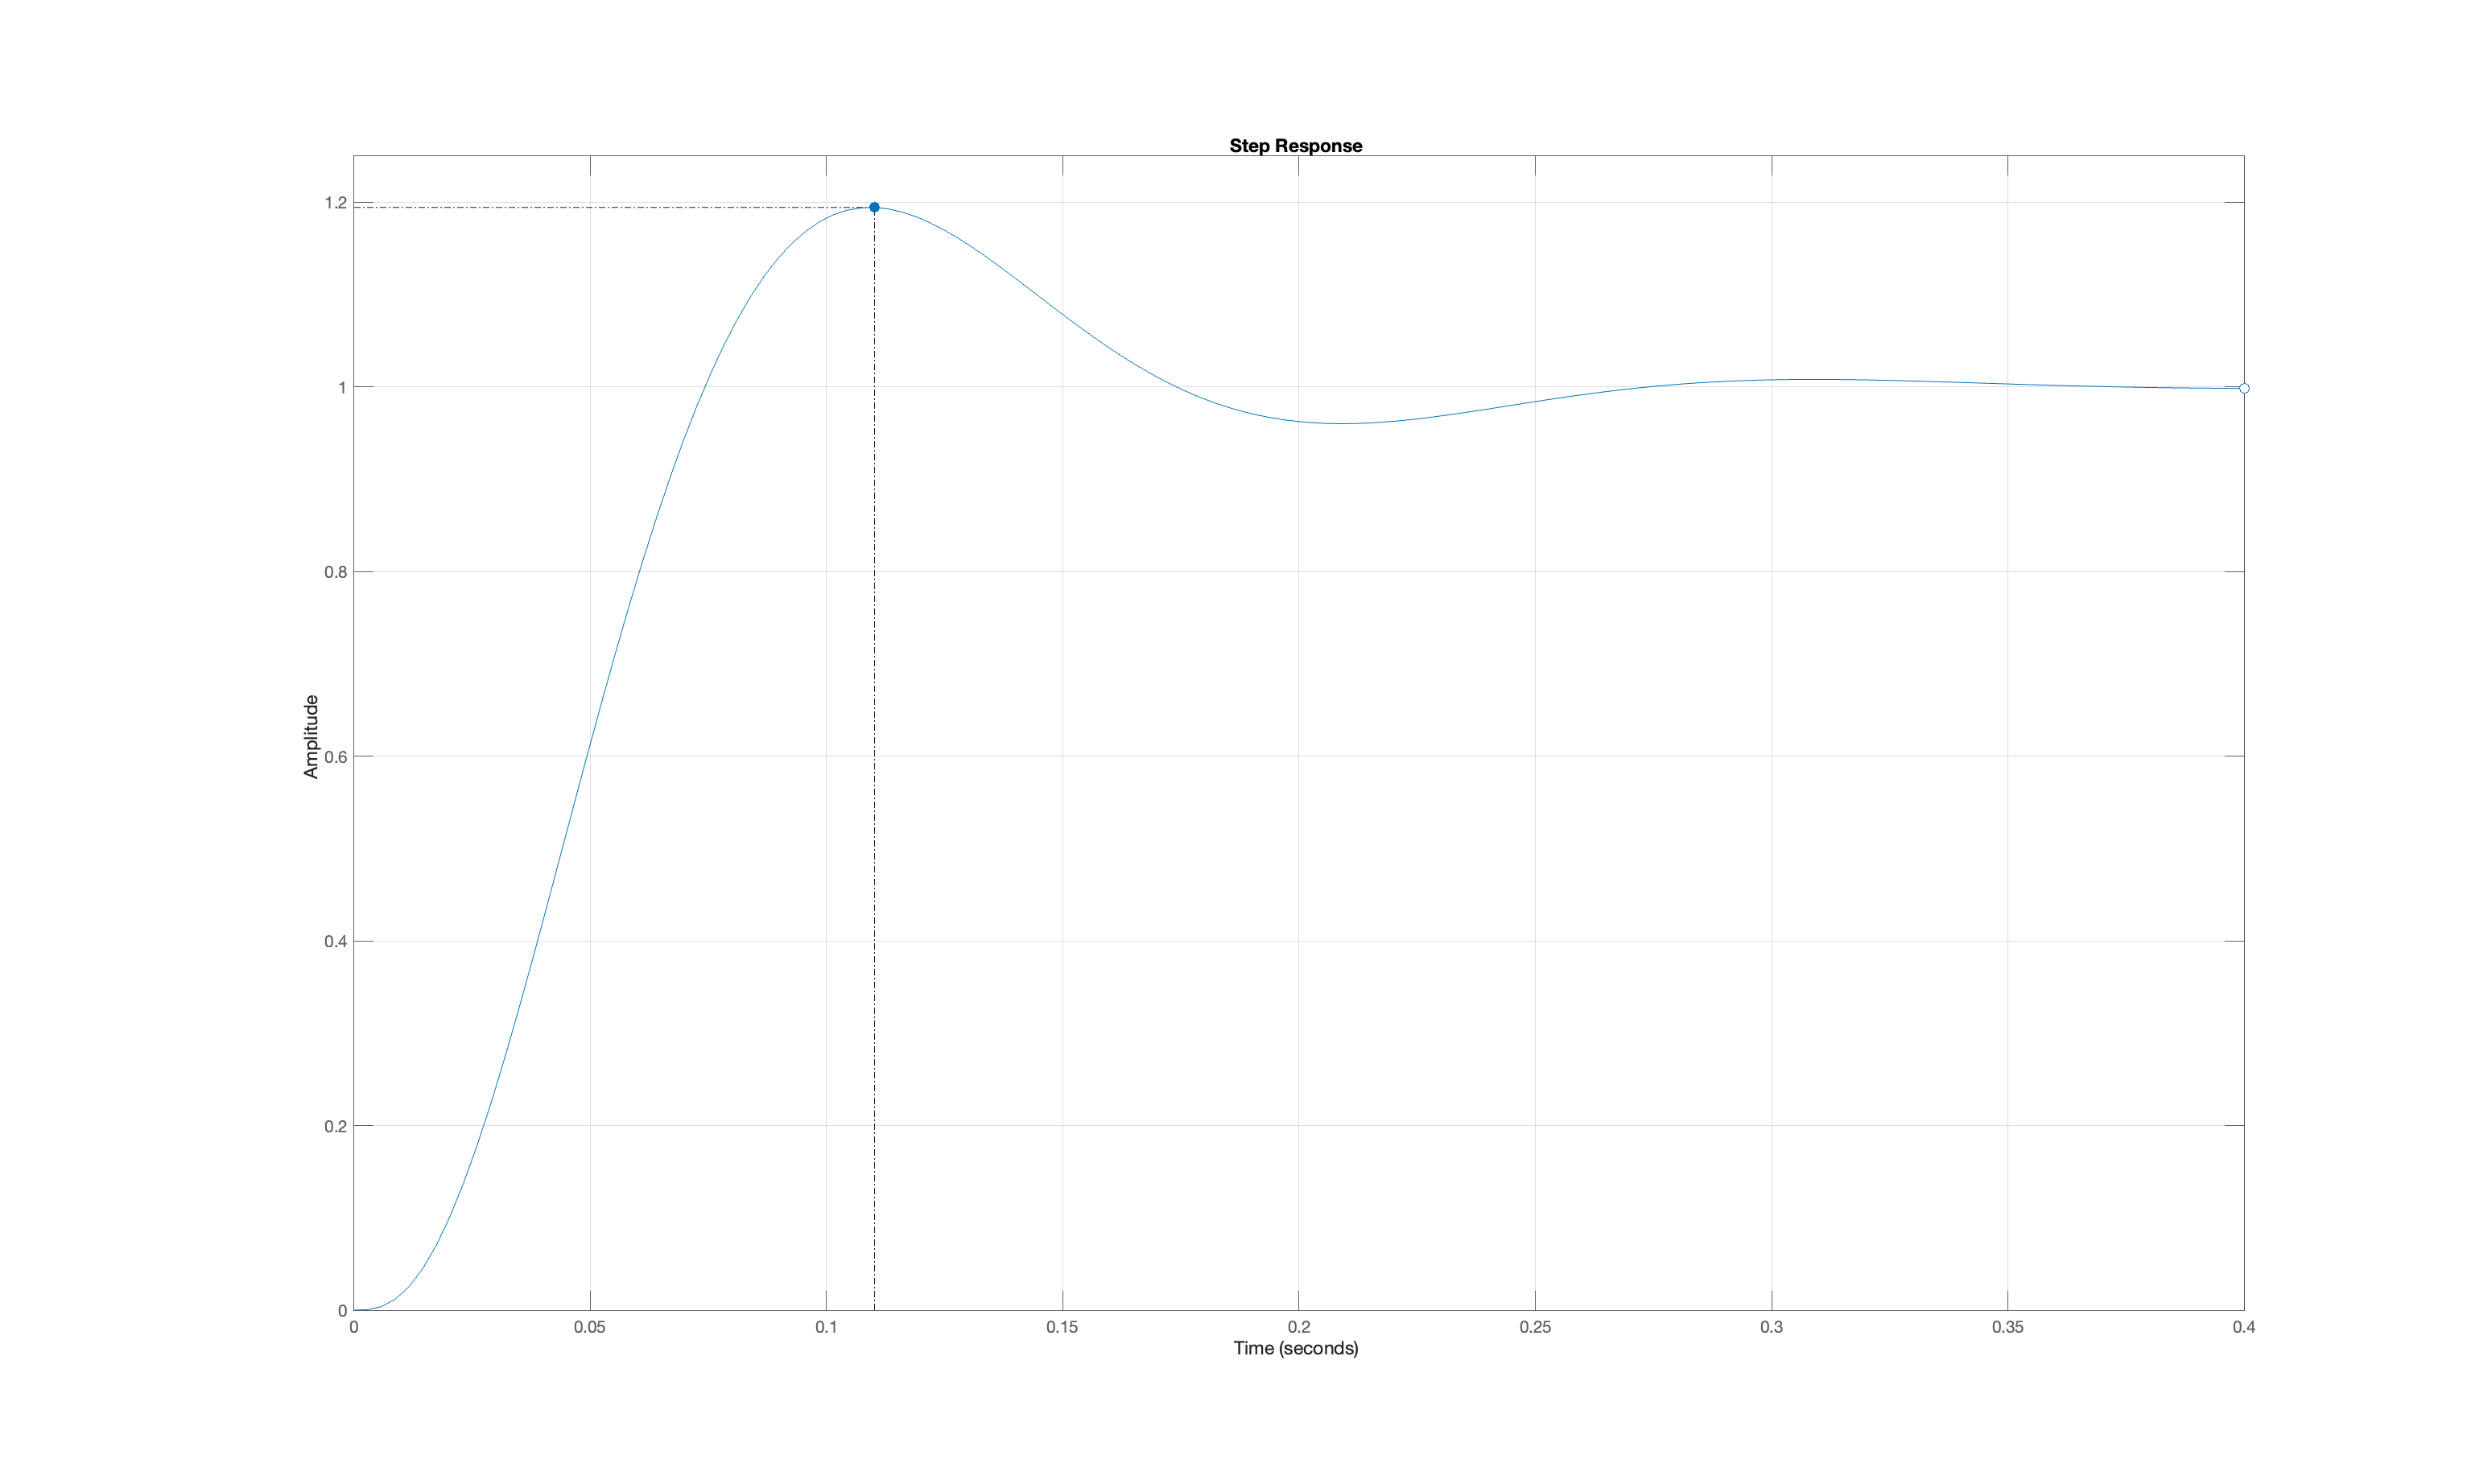
\includegraphics[clip, width=0.75\textwidth]{Step_Response.eps}
        \caption{Odezva na jednotkový skok}
        \label{fig:Unit_Step}
    \end{figure*}
\end{enumerate}

\newpage
\section{Příklad}
\begin{enumerate}[a)]
    \item Určení řádu astatismu\\
    Řád astatismu systému určím z počtu pólů v nule. Tento systém má v nulové frekvenci sklon 0 dB/dek z toho můžu určit astatismus řádu 0 systému\\
    - Obecně přenos otevřené smyčky: 
    \begin{align*}
        L(s) = K\frac{\prod(s+z_k)}{s^0\prod(s+p_k)}
    \end{align*}
    
    \item Konstanty ustáleného stavu
    \begin{align*}
        K_p &= \lim_{s \to 0} L(s) = \lim_{s \to 0} K\frac{\prod(s+z_k)}{s^0\prod(s+p_k)} = \left| \frac{K \prod(z_k)}{\prod(p_k)} \right| = konst.\\
        K_v &= \lim_{s \to 0} sL(s) = \lim_{s \to 0} sK\frac{\prod(s+z_k)}{s^0\prod(s+p_k)} = \left| 0\frac{K \prod(z_k)}{\prod(p_k)} \right| = 0\\
        K_a &= \lim_{s \to 0} s^2L(s) = \lim_{s \to 0} s^2K\frac{\prod(s+z_k)}{s^0\prod(s+p_k)} = \left| 0^2\frac{K \prod(z_k)}{\prod(p_k)} \right| = 0\\
    \end{align*}

    \begin{figure*}[h]
        \centering
        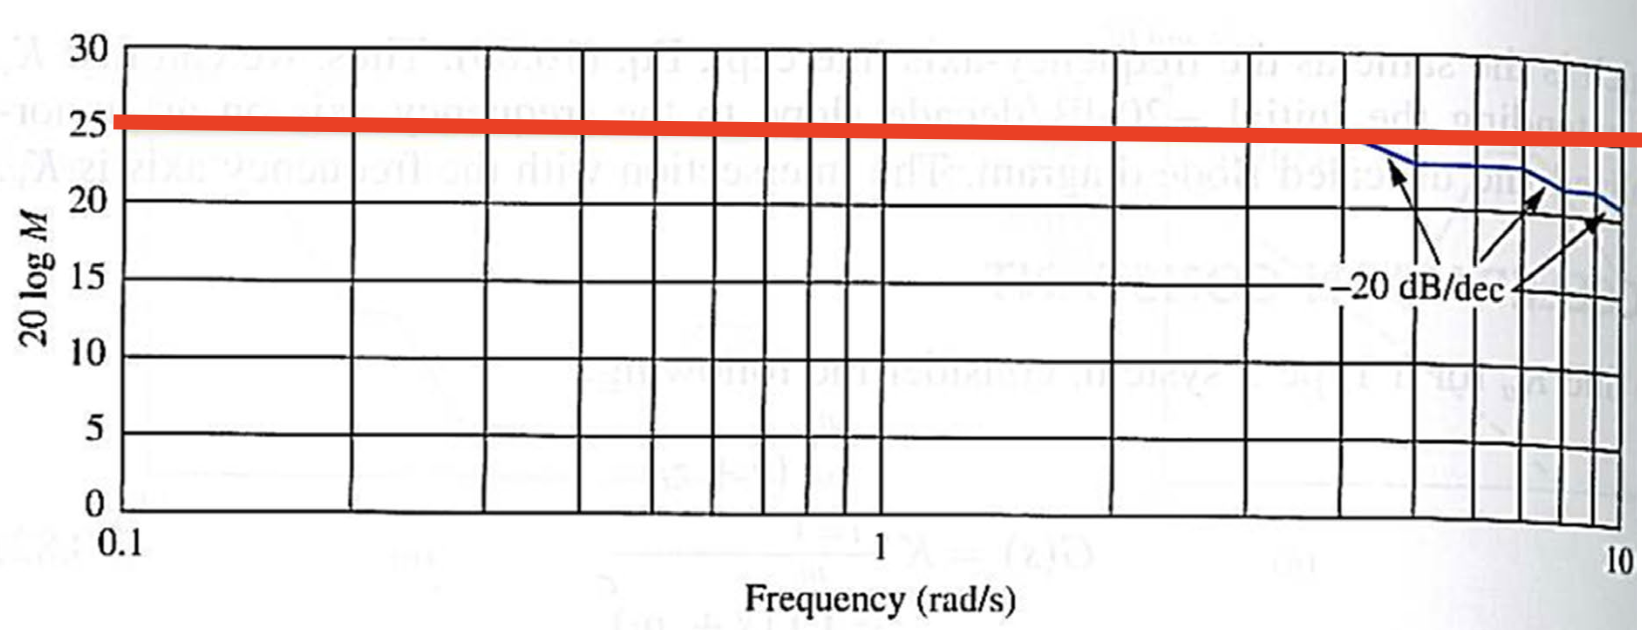
\includegraphics[clip, width=1.00\textwidth]{Konstanta rychlosti.png}
        \caption{Bodeho graf}
        \label{fig:Bode_plot}
    \end{figure*}
    - Konstantu $K_p$ z Bodeho grafu vyčtu pomocí proložení přímkou počáteční úsečky grafu. A tam kde přímka protne 0dB je hodnota rovna konstantě. V tomto případě je přímka rovnoběžná s frekvenční osou, tak jsem určil $K_p = \infty$

    \newpage
    \item Ustálené odchylky na:
    \[e_{ss} = \lim_{s\rightarrow 0} s \frac{r(s)}{1+L(s)}\]
    \begin{itemize}
        \item skok:
        \begin{align*}
            r(s) &= \frac{1}{s} & e_{ss,skok} &= \lim_{s\rightarrow 0} s \frac{r(s)}{1+L(s)} = \lim_{s\rightarrow 0} s \frac{\frac{1}{s}}{1+L(s)} = \frac{1}{1+K_p} = \frac{1}{\infty} = 0
        \end{align*}

        \item rampa:
        \begin{align*}
            r(s) &= \frac{1}{s^2} & e_{ss,rampa} &= \lim_{s\rightarrow 0} s \frac{r(s)}{1+L(s)} = \lim_{s\rightarrow 0} s \frac{\frac{1}{s^2}}{1+L(s)} = \frac{1}{0+K_v} = \frac{1}{0} = \infty
        \end{align*}

        \item parabola:
        \begin{align*}
            r(s) &= \frac{1}{s^3} & e_{ss,parabola} &= \lim_{s\rightarrow 0} s \frac{r(s)}{1+L(s)} = \lim_{s\rightarrow 0} s \frac{\frac{1}{s^3}}{1+L(s)} = \frac{1}{0+K_a} = \frac{1}{0} = \infty
        \end{align*}
    \end{itemize}
\end{enumerate}

\end{document}
